%%%%%%%%%%%%%%%%%%%%%%%%%%%%%%%%%%%%%%%%%%%%%%%%%%%
%% LaTeX book template                           %%
%% Author:  Amber Jain (http://amberj.devio.us/) %%
%% License: ISC license                          %%
%%%%%%%%%%%%%%%%%%%%%%%%%%%%%%%%%%%%%%%%%%%%%%%%%%%

%\documentclass[a4paper,11pt]{book}
\documentclass[b5paper,8pt]{book}
\usepackage{geometry}
\usepackage[T1]{fontenc}
\usepackage[utf8]{inputenc}
\usepackage{lmodern}
%%%%%%%%%%%%%%%%%%%%%%%%%%%%%%%%%%%%%%%%%%%%%%%%%%%%%%%%%
% Source: http://en.wikibooks.org/wiki/LaTeX/Hyperlinks %
%%%%%%%%%%%%%%%%%%%%%%%%%%%%%%%%%%%%%%%%%%%%%%%%%%%%%%%%%
\usepackage{hyperref}
\usepackage{graphicx}
\usepackage[english]{babel}

\usepackage{listings}
\usepackage{color}

\usepackage{algorithm}
\usepackage{algorithmic}

\usepackage{subfig}
\usepackage{amsmath}
\usepackage[makeroom]{cancel}

\usepackage{tcolorbox}

\usepackage{caption}

\usepackage[utf8]{inputenc}
\usepackage{imakeidx}
\usepackage{hyperref}

%\usepackage[spanish]{babel}
%\usepackage[usenames, dvipsnames]{color}
\definecolor{dkgreen}{rgb}{0,0.6,0}
\definecolor{gray}{rgb}{0.8,0.8,0.8}
\definecolor{mauve}{rgb}{0.58,0,0.82}
\definecolor{comments}{rgb}{1,1,0}

\lstset{frame=tb,
  language=C++,
  backgroundcolor=\color{white},
  aboveskip=3mm,
  belowskip=3mm,
  showstringspaces=false,
  columns=flexible,
  basicstyle={\scriptsize\ttfamily},
  numbers=none,
  numberstyle=\tiny\color{gray},
  keywordstyle=\color{blue},
  commentstyle=\color{dkgreen},
  stringstyle=\color{mauve},
  breaklines=true,
  breakatwhitespace=true
  tabsize=3
}

%%%%%%%%%%%%%%%%%%%%%%%%%%%%%%%%%%%%%%%%%%%%%%%%%%%%%%%%%%%%%%%%%%%%%%%%%%%%%%%%
% 'dedication' environment: To add a dedication paragraph at the start of book %
% Source: http://www.tug.org/pipermail/texhax/2010-June/015184.html            %
%%%%%%%%%%%%%%%%%%%%%%%%%%%%%%%%%%%%%%%%%%%%%%%%%%%%%%%%%%%%%%%%%%%%%%%%%%%%%%%%
\newenvironment{dedication}
{
   \cleardoublepage
   \thispagestyle{empty}
   \vspace*{\stretch{1}}
   \hfill\begin{minipage}[t]{0.66\textwidth}
   \raggedright
}
{
   \end{minipage}
   \vspace*{\stretch{3}}
   \clearpage
}

%%%%%%%%%%%%%%%%%%%%%%%%%%%%%%%%%%%%%%%%%%%%%%%%
% Chapter quote at the start of chapter        %
% Source: http://tex.stackexchange.com/a/53380 %
%%%%%%%%%%%%%%%%%%%%%%%%%%%%%%%%%%%%%%%%%%%%%%%%
\makeatletter
\renewcommand{\@chapapp}{}% Not necessary...
\newenvironment{chapquote}[2][2em]
  {\setlength{\@tempdima}{#1}%
   \def\chapquote@author{#2}%
   \parshape 1 \@tempdima \dimexpr\textwidth-2\@tempdima\relax%
   \itshape}
  {\par\normalfont\hfill--\ \chapquote@author\hspace*{\@tempdima}\par\bigskip}
\makeatother

%%%%%%%%%%%%%%%%%%%%%%%%%%%%%%%%%%%%%%%%%%%%%%%%%%%
% First page of book which contains 'stuff' like: %
%  - Book title, subtitle                         %
%  - Book author name                             %
%%%%%%%%%%%%%%%%%%%%%%%%%%%%%%%%%%%%%%%%%%%%%%%%%%%

% Book's title and subtitle
\title{\Huge \textbf{ Project Euler}  \\ \huge Solutions}
% Author
\author{\textsc{David Esparza Alba}}

\date{}

\makeindex

\begin{document}

\frontmatter
\maketitle

\tableofcontents

\mainmatter%%%%%%%%%%%%%%%%%%%%%%%%%%%%%%%%%%%%%%%%%%%%%%%%%%%%%%%
\addcontentsline{toc}{chapter}{80 - Square root digital expansion}
\chapter*{80 - Square root digital expansion}

\index{square root} 
It is well known that if the square root of a natural number is not an integer, then it is irrational. The decimal expansion of such square roots is infinite without any repeating pattern at all.\\

The square root of two is 1.41421356237309504880..., and the digital sum of the first one hundred decimal digits is 475.\\

For the first one hundred natural numbers, find the total of the digital sums of the first one hundred decimal digits for all the irrational square roots.\\

\section*{Solution}

To solve this problem we used the method of \textit{Square Root by Subtraction} described by Jarvis \cite{square_root}. This method allows us to find the square root of an integer $n$.\\

The algorithm \ref{alg:square_root} receives an integer $n$ and returns the first one hundred decimal digits of $\sqrt{n}$. The value of $p$ is set according of the number of decimal digits we want to calculate. 

\begin{algorithm}[H]
\caption{$squareRoot(n)$}
\begin{algorithmic}
    \STATE $a = 5n$
    \STATE $b=5$
    \STATE $p=10^{101}$
    \WHILE{$b < p$}
        \IF{$a \geq b$}
            \STATE $a \gets a-b$
            \STATE $b \gets b + 10$
        \ELSE
            \STATE $a \gets a \times 100$
            \STATE $b \gets \lfloor b/10 \rfloor \times 100 + 5$
        \ENDIF
    \ENDWHILE
    \STATE $b \gets \lfloor b/100 \rfloor$
    \RETURN b
\end{algorithmic}
\label{alg:square_root}
\end{algorithm}
 
\addcontentsline{toc}{chapter}{91 - Right triangles with integer coordinates}
\chapter*{91 - Right triangles with integer coordinates}

\index{binary search}
The points $P(x_1, y_1)$ and $Q(x_2, y_2)$ are plotted at integer co-ordinates and are joined to the origin, $O(0,0)$, to form $\Delta OPQ$.

\begin{figure}[H]
    \centering
    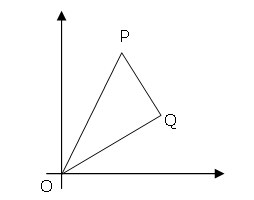
\includegraphics[scale=0.5]{images/pe911.png}
    \caption{}
    \label{fig:pe91a}
\end{figure}

There are exactly fourteen triangles containing a right angle that can be formed when each co-ordinate lies between 0 and 2 inclusive; that is, $0 \leq x1, y1, x2, y2\leq 2$.

\begin{figure}[H]
    \centering
    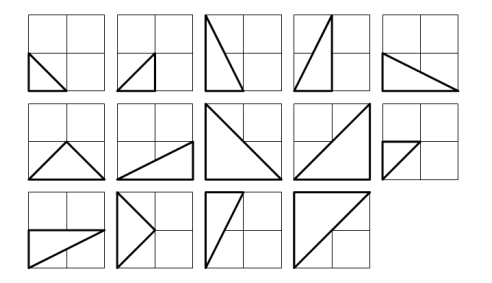
\includegraphics[scale=0.5]{images/pe912.png}
    \caption{}
    \label{fig:pe91b}
\end{figure}

Given that $0 \leq x1, y1, x2, y2 \leq 50$, how many right triangles can be formed?

\section*{Solution}

Since the coordinates are integer numbers in the range of $[0,50]$, a brute force approach will run in $O(n^4)$, with $n=50$ we are talking around six millions of operations, which looks reasonable to run in less than a minute. Now, in order to improve a little bit the running time we will do the following:

\begin{enumerate}
    \item Place the first point $(x_1,y_1)$ in the grid. This will take $O(n^2)$ to go trough the whole grid.
    \item For the other point $(x_2,y_2)$ iterate trough all values in the $y-axis$ and using a binary search obtain the $x-coordinate$, this part will run in $O(n \log n)$. Avoid to count the points where $y_2 = y_1$ and those where $x_2 = x_1$. To identify if we have found a valid coordinate we must check that the following statement is true (cosine law).
    
    $$
    x_1^2 + y_1^2 + (x_2-x_1)^2 + (y_2-y1)^2 - x_2^2 - y_2^2 = 0
    $$
    
    \item After counting the triangles f in step 2, we just need add $3n^2$, which is the number of right triangles with sides parallel to the $x$ and $y$ axis. 
    
\end{enumerate}

The running time of this solution is $O(n^3 \log n)$, which is around $7 \times 10^5$ operations.
\addcontentsline{toc}{chapter}{94 - Almost equilateral triangles}
\chapter*{94 - Almost equilateral triangles}

\index{triangle area}
It is easily proved that no equilateral triangle exists with integral length sides and integral area. However, the almost equilateral triangle 5-5-6 has an area of 12 square units.\\

We shall define an almost equilateral triangle to be a triangle for which two sides are equal and the third differs by no more than one unit.\\

Find the sum of the perimeters of all almost equilateral triangles with integral side lengths and area and whose perimeters do not exceed one billion ($10000000000$).\\

\section*{Solution}

Two sides of the triangle are equal and the other differs by no more than one unit. One option is having lengths: $k,k,k+1$. Using the Heron's formula to obtain the triangle's area we have:

\begin{align*}
    s &= \frac{k + k + k+1}{2} \\
    &= \frac{3k+1}{2}
\end{align*}

and the triangle's area is given by

\begin{align*}
    A_1 &= \sqrt{s(s-k)(s-k)(s-k-1)}\\
    &= \sqrt{\left ( \frac{3k+1}{2} \right ) \left ( \frac{k+1}{2} \right ) \left ( \frac{k+1}{2} \right ) \left ( \frac{k-1}{2} \right )}\\
    &= \frac{(k+1) \sqrt{3k^2 - 2k - 1}}{4}
\end{align*}

For lengths $k,k,k-1$ and following the same process we obtain that the area is 

$$
A_2 = \frac{(k-1) \sqrt{3k^2 + 2k - 1}}{4}
$$

Basically we are looking for values of $k$ such as $3k^2 \pm 2k - 1$ is a square number, and that $(k \mp 1)(3k^2 \pm 2k - 1)$ is divisible by 4.\\

After generating the fist values of $k$ I noticed that they are of the form $4i+1$, for some positive integers values of $i$. The upper bound for $k$ is $k \leq M$, where $M = (10^9-1)/3$. So i started iterating trough all values of the form $4i+1$, for $i=1, \ldots, M/4-1$ and checked if $3k^2 \pm 2k - 1$ was a square number, and if it was I added $3k \mp 1$ (the perimeter) to the result. The program ran in about $1.4$ seconds in \texttt{C++}.
\addcontentsline{toc}{chapter}{95 - Amicable chains}
\chapter*{95 - Amicable chains}

\index{prime numbers}
The proper divisors of a number are all the divisors excluding the number itself. For example, the proper divisors of 28 are 1, 2, 4, 7, and 14. As the sum of these divisors is equal to 28, we call it a perfect number.\\

Interestingly the sum of the proper divisors of 220 is 284 and the sum of the proper divisors of 284 is 220, forming a chain of two numbers. For this reason, 220 and 284 are called an amicable pair.\\

Perhaps less well known are longer chains. For example, starting with 12496, we form a chain of five numbers:

$$
12496 \rightarrow 14288 \rightarrow 15472 \rightarrow  14536 \rightarrow  14264  (\rightarrow  12496 \rightarrow  ...)
$$

Since this chain returns to its starting point, it is called an amicable chain.\\

Find the smallest member of the longest amicable chain with no element exceeding one million.

\section*{Solution}

For a number $n$ the sum of the divisors less or equal than $n$ is given by

$$
S(n) = \prod_{i=1}^m \frac{p_i^{k_i+1} - 1}{p_i - 1}
$$

where 

$$
n = \prod_{i=1}^m p_i^{k_i}
$$

To generate the primes up to $10^6$ quickly we can use the \textit{Sieve of Eratosthenes}.\\

The idea is to mark the elements in a sequence and if we found a number that is already marked we will be able to obtain the length of the sequence and the starting/ending point of the cycle. We used an array $L$ and a counter to obtain the length of a cycle. For the example mentioned in the description we will have

\begin{align*}
    L_{12496} = 1 \\
    L_{14288} = 2 \\
    L_{15472} = 3 \\
    L_{14536} = 4 \\
    L_{14264} = 5
\end{align*}

The next value is $12496$ which is already marked, and the value of the counter is $6$, so the length of the sequence is $6 - L_{12496} = 5$. Also we can store in another array $X$ the starting/ending point of the cycle in each element of the chain, this is easily done using a recursive function.

\begin{align*}
    X_{12496} = 12496 \\
    X_{14288} = 12496 \\
    X_{15472} = 12496 \\
    X_{14536} = 12496 \\
    X_{14264} = 12496
\end{align*}

Sometimes we can start in a number that will led us to an already found cycle, just avoid counting the numbers found before entering the cycle.\\

Finally we just need to look for the number $k$ which $k = X_k$, and have the greatest $L_k$. Start moving trough that cycle to find the smallest element.
\addcontentsline{toc}{chapter}{98 - Anagramic squares}
\chapter*{98 - Anagramic squares}

\index{hash-map} \index{anagrams}
By replacing each of the letters in the word CARE with 1, 2, 9, and 6 respectively, we form a square number: $1296 = 36^2$. What is remarkable is that, by using the same digital substitutions, the anagram, RACE, also forms a square number: $9216 = 96^2$. We shall call CARE (and RACE) a square anagram word pair and specify further that leading zeroes are not permitted, neither may a different letter have the same digital value as another letter.\\

Using \texttt{words.txt} (right click and 'Save Link/Target As...'), a 16K text file containing nearly two-thousand common English words, find all the square anagram word pairs (a palindromic word is NOT considered to be an anagram of itself).\\

What is the largest square number formed by any member of such a pair?\\

NOTE: All anagrams formed must be contained in the given text file.\\

\section*{Solution}

The longest word in the file has 14 letters, but looking for the anagram pairs I found out that the longest word with an anagram pair has 10 letters. So we only need to iterate through numbers less than $10^5$ and store their squares (only the ones that has anagrams). For that I used a matrix, and in row 1 I stored the 1-digit squares, in row 2 the 2-digit squares, and so on.\\

To find words that are anagram pairs I used a map with the sorted word as key, because if we sort two anagrams we get the same string, and they will have the same key. The same approach is done to find the anagram squares, sort the digits and convert the resulting number into a string, with the leading zeros included, and use that string as key of a map, that help us to identify anagram squares.\\

I stored all the anagram pairs in a vector of pairs. For each pair $<A,B>$ I obtained the length of the words and started searching in the matrix in the corresponding row. For each number I checked  if that number and word $A$ were a valid match, for that I used two arrays, in one I was marking the digits that were already being used, and in the other array I stored the digit assigned to each letter. Doing that I could check that two letters didn't have the same digit assigned and also that one letter didn't have two different digits assigned.\\

Once we know the numeric value of each letter we build a new number using word $B$ of the pair, and search for that number in the same row of the matrix, if the numbers are sorted we can use a binary search. If the number is found, then that pair is an \textit{anagram word pair}. We repeat the process for each pair of words and report the largest square found. This approach run in $0.4$ seconds approximately. 
\addcontentsline{toc}{chapter}{100 - Arranged probability}
\chapter*{100 - Arranged probability}

\index{Diophantine quadratic}
If a box contains twenty-one coloured discs, composed of fifteen blue discs and six red discs, and two discs were taken at random, it can be seen that the probability of taking two blue discs, $P(BB) = (15/21)(14/20) = 1/2$.\\

The next such arrangement, for which there is exactly 50\% chance of taking two blue discs at random, is a box containing eighty-five blue discs and thirty-five red discs.\\

By finding the first arrangement to contain over $10^{12} = 1000000000000$ discs in total, determine the number of blue discs that the box would contain.

\section*{Solution}

Be $x$ the number of blue discs, and $y$ the total number of discs. We are looking values of $x$ and $y$ such as

\begin{align*}
    \left ( \frac{x}{y} \right ) \left ( \frac{x-1}{y-1} \right ) = \frac{1}{2} \\
    2x^2 - 2x = y^2 - y \\
    2x^2 - 2x - y^2 + y = 0
\end{align*}

A Diophantine equation is a polynomial equation with integer solutions only. A linear Diophantine equation is

$$
ax + by = c.
$$

Which can be solved using the \textit{Extended Euclidean} algorithm. For our case we have a quadratic Diophantine equation, and according to Mario Alpern's explanation \cite{quadratic_diophantine}, an equation of the form

$$
 ax^2 + bxy + cy^2 + dx + ey + f = 0
$$

has the following solutions:

\begin{align*}
    x_{n+1} &= Px_n + Qy_n + K \\
    y_{n+1} &= Rx_n + Sy_n + L
\end{align*}

For our specific equation the values of $P,Q,K,R,S,L$ are:

\begin{align*}
    P &= 3 \\
    Q &= 2 \\
    K &= -2 \\
    R &= 4 \\
    S &= 3 \\
    L &= -3
\end{align*}

The explanation of why these values is detailed in Mario Alpern's site.\\

Coming back to our problem. Using the formulas mentioned above, we only need to iterate though the different value of $x$ and $y$ until $y$ exceeds $10^{12}$.


\addcontentsline{toc}{chapter}{101 - Optimum polynomial}
\chapter*{101 - Optimum polynomial}

\index{least squares}
If we are presented with the first k terms of a sequence it is impossible to say with certainty the value of the next term, as there are infinitely many polynomial functions that can model the sequence.\\

As an example, let us consider the sequence of cube numbers. This is defined by the generating function, 
$u_n = n^3: 1, 8, 27, 64, 125, 216, \cdots$\\

Suppose we were only given the first two terms of this sequence. Working on the principle that ''simple is best'' we should assume a linear relationship and predict the next term to be 15 (common difference 7). Even if we were presented with the first three terms, by the same principle of simplicity, a quadratic relationship should be assumed.\\

We shall define $OP(k, n)$ to be the $n^{th}$ term of the optimum polynomial generating function for the first $k$ terms of a sequence. It should be clear that $OP(k, n)$ will accurately generate the terms of the sequence for $n \leq k$, and potentially the first incorrect term (FIT) will be $OP(k, k+1)$; in which case we shall call it a bad $OP (BOP)$.\\

As a basis, if we were only given the first term of sequence, it would be most sensible to assume constancy; that is, for $n \geq 2, OP(1, n) = u_1$.\\

Hence we obtain the following OPs for the cubic sequence:

\begin{align*}  
    OP(1, n) &= 1 \hphantom{4} (1, \textcolor{red}{1}, 1, 1, \ldots) \\
    OP(2, n) &= 7n-6 \hphantom{4} (1, 8, \textcolor{red}{15}, \ldots) \\
    OP(3, n) &= 6n^2-11n+6 \hphantom{4} (1, 8, 27, \textcolor{red}{58}, \ldots) \\
    OP(4, n) &= n^3 \hphantom{4} (1, 8, 27, 64, 125, \ldots) \\
\end{align*}

Clearly no BOPs exist for $k \geq 4$.\\

By considering the sum of FITs generated by the BOPs (indicated in red above), we obtain 1 + 15 + 58 = 74.\\

Consider the following tenth degree polynomial generating function:

$$
u_n = 1 - n + n^2 - n^3 + n^4 - n^5 + n^6 - n^7 + n^8 - n^9 + n^{10}
$$

Find the sum of FITs for the BOPs.

\section*{Solution}

We are asked to obtain a polynomial model of degree $k-1$ $(1 \leq k \leq 10)$ that fits the first $k$ elements of $u_n$ $(u_1, u_2, \ldots, u_k)$ exactly, and then evaluate the polynomial model using the element $k+1$, and add the result to the answer.\\

Starting from the fact that if we have $n+1$ points, a polynomial of degree $n$ will cross all points. In practice that is called \textit{over-fitting}, and happens when the model is to complex to fit the data, and when we evaluate the model with other points, is possible that we get a larger error.\\

Then for $k$ points, the polynomial model of degree $k-1$ we have to obtain has the following form:

$$
OP(k,n) = \theta_0 + \theta_1n_1 + \theta_2n^2 + \cdots + \theta_{k-1}n^{k-1}
$$

We need to find the values of $\theta$, and then evaluate $OP(k,n)$ in $k+1$.\\

The equation above can be seen as a \textit{linear model} of the form:

$$
OP(k,n) = \theta_0f_0(n) + \theta_1f_1(n) + \theta_2f_2(n) + \cdots + \theta_{k-1}f_{k-1}(n)
$$

So we can use the \textit{Least Squares} method to obtain the value of $\theta$ and get

$$
\theta = (X^TX)^{-1}X^T y
$$

where $y$ are the values of $u_n$, and $X$ is a matrix with element $X_{i,j}$ representing $f_j(i)$.\\

There are programming languages that have functions that estimates the value of $\theta$. In my case I used \texttt{R}, which have the function \texttt{lm} that estimates the value of $\theta$, and \texttt{predict}, which evaluates a model in a given point.
\addcontentsline{toc}{chapter}{104 - Pandigital Fibonacci ends}
\chapter*{104 - Pandigital Fibonacci ends}

\index{Fibonacci} \index{logarithms}

The Fibonacci sequence is defined by the recurrence relation:\\

$$
F_n = F_{n-1} + F_{n-2}, \mbox{where} \hphantom{4} F_1 = 1 \mbox{ and } F_2 = 1.
$$

It turns out that $F_{541}$, which contains 113 digits, is the first Fibonacci number for which the last nine digits are 1-9 pandigital (contain all the digits 1 to 9, but not necessarily in order). And $F_{2749}$, which contains 575 digits, is the first Fibonacci number for which the first nine digits are 1-9 pandigital.\\

Given that $F_k$ is the first Fibonacci number for which the first nine digits AND the last nine digits are 1-9 pandigital, find k.

\section*{Solution}

Obtaining the last 10 digits of a Fibonacci number is not a problem, in fact you can store the last 10 digits only and ignore the rest, but what about the first 10 digits? Well for this case we used the \textit{Binet's Formula} which states that

$$
F_n = \frac{\phi^n - (1 - \phi)^{n}}{\sqrt{5}}
$$

where $\phi$ is the golden ratio and is defined by

$$
\phi = \frac{1 + \sqrt{5}}{2} \approx 1.6180339887 \ldots
$$

Since the value of $(1 - \phi)^n$ is getting smaller as $n$ increases we can redefine the equation as

$$
F_n = \left [ \frac{\phi^n}{\sqrt{5}} \right ]
$$

What we did was to generate some Fibonacci numbers, after that only kept track of the first 10 and the last 10 digits. The first $k$ digits of a number $n$ can be obtained with the following formula:

$$
10^{\log{n} - k + 1}
$$

Then

\begin{align*}
    \log{F_n} &= \log{\frac{\phi^n}{\sqrt{5}}} \\ 
    &= n \log{\phi} - 0.5\log{5}
\end{align*}

Finally, once we have the first 10 digits and the last 10 digits we only need to check if both are pandigital, which can be easily verified, and this way we avoid the use of big numbers and all the carry operations.
\addcontentsline{toc}{chapter}{206 - Concealed Square}
\chapter*{206 - Concealed Square}

\index{brute force}
Find the unique positive integer whose square has the form $1\_2\_3\_4\_5\_6\_7\_8\_9\_0$,
where each '''\_' is a single digit.

\section*{Solution}

I'm not very happy with my solution here, but here it is. The first thing to notice is that we are looking for 9 digits between $[0,9]$, making $10^9$ possible combinations. Now, the number we are looking must have 10 digits and has the form:

$$
d_0d_1d_2d_3d_4d_5d_6d_7d_8d_9.
$$

We know that $d_9^2$ must ends with $0$. So the only choice is that

$$
d_9 = 0
$$

Also we know that 

$$
d_8^2 + d_7d_9 = 9
$$

Replacing $d_9$ with 0 we obtain

$$
d_8^2 = 9
$$

We have two solutions here, $d_8$ can be 3, or 7. What I did was to try both numbers, and give $d_7$ different values.\\

With the values of $d_7,d_8$, and $d_9$, we can find the the other seven digits by brute force in a reasonable amount of time. 
\addcontentsline{toc}{chapter}{323 - Bitwise-OR operations on random integers}
\chapter*{323 - Bitwise-OR operations on random integers}

\index{probability}
Let $y_0, y_1, y_2, \ldots$ be a sequence of random unsigned 32 bit integers
(i.e. $0 \leq y_i < 2^{32}$, every value equally likely).\\

For the sequence $x_i$ the following recursion is given:

\begin{align*}
    x0 &= 0 \mbox{ and} \\
    x_i &= x_{i-1}|y_{i-1}, \mbox{ for } i > 0. ( \hphantom{2} | \mbox{ is the bitwise-OR operator})
\end{align*}

It can be seen that eventually there will be an index $N$ such that $xi = 2^{32} -1$ (a bit-pattern of all ones) for all $i \geq N$.\\

Find the expected value of N. 
Give your answer rounded to 10 digits after the decimal point.

\section*{Solution}

We can see this as a game where the player wins when all 32 bits are 1. Define $s^{(t)}$ as the number of bits set to $1$ after t games, and lets call $P_i^{(t)}$ the probability of having $i$ 1's after $t$ games. Initially we have that $P_i^{(1)}$ follows a binomial distribution

$$
P_i^{(1)} = P(s^{(1)}=i) = \binom{32}{i} (0.5)^i (0.5)^{32-i}
$$

since all bits are equally likely, the probability for a bit of having a value of 0 is $0.5$.\\

Is important to notice that there will be at least one attempt, so $P(N=1) = 1$.\\

Let's assume we did not win in the first attempt. All the bits set to 1 in the first attempt will remain as 1 (because of the bitwise-OR), and there is a chance  that more bits are set to 1 in the second attempt, but the amount of 1's wont decrease.\\

We need to calculate the conditional probability of getting $i$ ones, given that until the last attempt we had $j$ ones. We will call this probability $Q_{ij}$ $(i \geq j)$.\\

To calculate the value of $Q_{ij}$ we know from the last attempt that $j$ from the 32 bits are 1, and the other $32-j$ bits are 0's. First we are going to place $i-j$ new bits to 1 (bits that were 0 after the last attempt). This follows a binomial distribution and we will call it $q_a$ and is given by

$$
q_a = \binom{32-j}{k} (0.5)^k (0.5)^{32-j-k},
$$

where $k = i-j$.\\

We still need to deal with the bits that were 1 after the previous attempt. Well those bits don't matter if they are 0 or 1 in the next attempt, at the end they will remain with the value of 1. Be $q_b$ the probability of getting at most $j$ 1's in the next attempt in those bits. Its value is defined by

$$
q_b = \sum_{h=1}^j \binom{j}{h} (0.5)^h(0.5)^{j-h}.
$$

Then the value of $Q{ij}$ is defined as

$$
Q_{ij} = q_a q_b
$$

Once we know each value of $Q_{ij}$, the new value of $P^{(t+1)}_i$ is obtained by the formula of total probability:
 
\begin{align*}
P^{(t+1)}_i &= P(s^{(t+1)}=i)\\
&= P(s^{(t+1)}=i|s^{(t)}=0)P(s^{(t)}=0) + \cdots + P(s^{(t+1)}=i|s^{(t)}=i)P(s^{(t)}=i)\\
&= \sum_{j=0}^i P(s^{(t+1)}=i|s^{(t)}=j)P(s^{(t)}=j) \\
&= \sum_{j=0}^i Q_{ij} P^{(t)}_j
\end{align*}

The probability of keep playing (probability of losing) is given by $1 - P_{32}$. As we continue playing that value will approach to zero. If we continuously add that value we will find the value of $E(N)$. Then

\begin{align*}
    E_1 &= 1 \\
    E_i &= E_{i-1} + (1 - P_{32}^{(i)}) \mbox{ for } i \geq 2
\end{align*}


\addcontentsline{toc}{chapter}{345 - Matrix Sum}
\chapter*{345 - Matrix Sum}

\index{Hungarian algorithm}
We define the Matrix Sum of a matrix as the maximum sum of matrix elements with each element being the only one in his row and column. For example, the Matrix Sum of the matrix below equals 3315 ( = 863 + 383 + 343 + 959 + 767):

\begin{figure}[H]
    \centering
    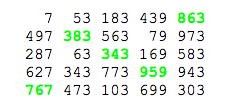
\includegraphics[scale=0.5]{images/pe345a.png}
    \caption{Caption}
    \label{fig:pe345a}
\end{figure}


Find the Matrix Sum of:

\begin{figure}[H]
    \centering
    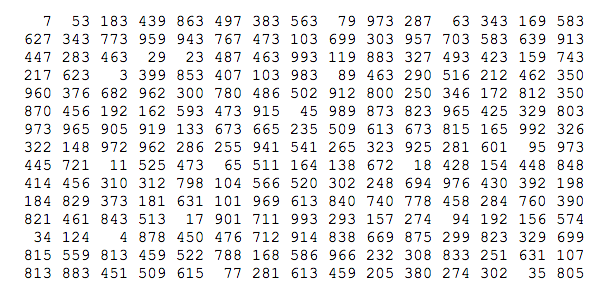
\includegraphics[scale=0.5]{images/pe345b.png}
    \caption{Caption}
    \label{fig:pe345b}
\end{figure}


\section*{Solution}

This problem can be seen as a Minimum Bipartite Matching Problem. From one side we have the rows, and in the other side we have the columns, and we must find the minimum 1-1 matching. In other words, for each row we must assign only one column, and the sum of all matches must be minimum.\\

For this problem we can use \textit{Hungarian Algorithm}, which if my memory is correct runs in $O(n^4)$, where $n$ is the size of the matrix. In \cite{hungarian} there is a great explanation of the algorithm.


\addcontentsline{toc}{chapter}{357 - Prime generating integers}
\chapter*{357 - Prime generating integers}

\index{prime numbers}
Consider the divisors of $30: 1,2,3,5,6,10,15,30$.
It can be seen that for every divisor $d$ of $30$, $d+30/d$ is prime\\.

Find the sum of all positive integers $n$ not exceeding $100000000$
such that for every divisor $d$ of $n$, $d+n/d$ is prime.

\section*{Solution}

The sequences for the first ten numbers are the following:

\begin{align*}
    2 &: 3,3\\
    3 &: 4,4\\
    4 &: 5,4,5\\
    5 &: 6,6\\
    6 &: 7,5,5,7\\
    7 &: 8,8\\
    8 &: 9,6,6,9\\
    9 &: 10,6,10\\
    10 &: 11,7,7,11
\end{align*}

Is easy to notice that the first element in the sequence is $n+1$, then $n+1$ must be prime. Then the integers we are looking are even, since $n+1$ must be prime, and all prime numbers except $2$ are odd.\\

So far we know that we are looking for even numbers, and since all even numbers have $2$ as a divisor, then $n/2+2$ must be prime as well. Then we are looking even numbers such as, $n+1$ is prime and $n/2 + 2$ is prime.\\

I found out (by try and error) that these integers, except $2$ and $6$ ,are of the form of $10 + 20a, 18+20b$, and $22+20c$, for $a,b,c \geq 0$.  Now, not every number is valid, so we must check if all divisors $d$ of those numbers meet that $d + n/d$ is prime. From sequences above we can notice the sequences are mirrored from half, then we only need to search for divisors up to $\sqrt{n}$, which will run a lot faster.   
\addcontentsline{toc}{chapter}{381 - (prime-k) factorial}
\chapter*{381 - (prime-k) factorial}

\index{Extended Euclidean} \index{inverse multiplicative} \index{modular arithmetic} \index{Wilson's theorem}

For a prime $p$ let $S(p) = \left ( \sum_{k=1}^5(p-k)! \right ) \bmod{p}$.\\

For example, if $p=7$,

\begin{align*}
    \sum_{k=1}^5(p-k)! &= (7-1)! + (7-2)! + (7-3)! + (7-4)! + (7-5)!\\
    &= 6! + 5! + 4! + 3! + 2!\\
    &= 720+120+24+6+2\\
    &= 872.
\end{align*}


As $872 \bmod{7}$ = 4, $S(7) = 4$.\\

It can be verified that $\sum_{p=5}^{99} S(p) = 480$.\\

Find $\sum_{p=5}^{10^8} S(p)$.

\section*{Solution}

By doing simple math and using modular arithmetic we get the $S(p)$ is defined by

\begin{align*}
    S(p) &= \left ( (p-5)! \bmod p \right ) \times 9 \\
    &= \left ( \left ( \frac{(p-1)!}{(p-1)(p-2)(p-3)(p-4)} \right ) \bmod p \right ) \times 9
\end{align*}

According to Wilson's Theorem \cite{wilson_theorem},

$$
(n-1)! \bmod n = -1 \bmod p
$$

Then, we only need to get rid of the denominator by using modular arithmetic. More precisely by using the inverse multiplicative. Suppose we have the following operation

$$
\frac{a}{b} \bmod m
$$

we can rewrite it as

$$
\left ( a \bmod m \right ) \left ( \frac{1}{b} \bmod m \right )
$$

The inverse multiplicative of $b$ is a number $k$, such that $(bk) \bmod n = 1$. Getting back to our problem, we are looking for an integer $k$ such that

$$
k(p-1)(p-2)(p-3)(p-4) \bmod p = 1
$$

Using modular arithmetic we have that

\begin{align*}
    (k(-1)(-2)(-3)(-4)) \bmod p &= 1 \\
    24k \bmod p &= 1
\end{align*}

Then 

\begin{align*}
    S(p) &= \left ( \frac{(p-1)!}{24} \bmod{p} \right ) \times 9 \\
    &= \left ( (p-1)! \frac{3}{8} \right ) \bmod p \\
    &= (-1 \bmod p) (3k \bmod p) \\
    &= (-3 \bmod p) (k \bmod p)\\
    &= (p-3)(k \bmod p)
\end{align*}

where $8k \bmod p = 1$\\

The value of $k$ can be found using the \textit{Extended Euclidean Algorithm}, which finds the inverse multiplicative of a number $a \bmod n$, only when $a$ and $n$ are coprimes. Since for our problem $n$ is prime, we can use it.\\

The \textit{Extended Euclidean Algorithm} find the values of $x$ and $y$ that solve the following equation:

$$
ax + by = 1
$$

Using $a=8$ and $b=p$ we have

$$
8x + py = 1
$$

Obtaining the modulus in both sides of the equation we get

\begin{align*}
    (8x + py) \bmod p &= 1 \\
    8x \bmod p &= 1
\end{align*}

which is what we are looking for. So basically we must calculate the value of $x$ using the \textit{Extended Euclidean Algorithm} and add the value of $p$ to avoid negative values. Then

$$
(x,y) = \mbox{ExtendenEuclidean}(8,p)
$$

and

$$
k = \left (x + p \right ) \bmod p
$$

Finally the value of $S(p)$ is given by

$$
S(p) = \left ( (p-3) \times k \right ) \bmod p
$$
\addcontentsline{toc}{chapter}{429 - Sum of squares of unitary divisors}
\chapter*{429 - Sum of squares of unitary divisors}

\index{prime numbers} \index{sum of combinations of products}
A unitary divisor $d$ of a number $n$ is a divisor of $n$ that has the property $gcd(d, n/d) = 1$.
The unitary divisors of $4! = 24$ are $1$, $3$, $8$ and $24$.
The sum of their squares is $1^2 + 3^2 + 8^2 + 24^2 = 650.$ \\

Let $S(n)$ represent the sum of the squares of the unitary divisors of $n$. Thus $S(4!)=650$. \\

Find $S(100000000!)$ modulo $1000000009$.

\section*{Solution}

First of all we must avoid calculating $n!$ directly. A better approach is to represent $n!$ as the product of its prime factors. For example, for $4!$ we have

$$
4! = 2^3 \times 3^1.
$$

Since we only care about those divisors with $gcd(d,n/d) = 1$, we must represent the number as the product of factors with exponent $1$. For $4!$ we obtain

$$
4! = 8^1 \times 3^1.
$$

The result we are looking for is the sum of the products of all combinations of the square of those factors. For this specific case we have that

$$
S(4!) = 1 + 8^2 + 3^2 + 8^2 3^2 = 650
$$

To calculate that sum we can use the following trick. Suppose there $3$ factors, $f_1, f_2, f_3$. The sum of the products of all combinations of those factors is given by:

$$
(1 + f_1)(1 + f_2)(1 + f_3) = 1 + f_1 + f_2 + f_3 + f_1f_2 + f_1f_3 + f_2f_3 + f_1f_2f_3.
$$

For our problem, if we have $m$ factors the solution would be given by

\begin{align*}
    S(n!) &= \prod_{i=1}^m (1 + f_i^2)\\
    &= \prod_{i=1}^m (1 + p_i^{2k_i}) 
\end{align*}


To obtain the value of $p_i^{2k^i}$ we can use binary exponentiation, in that case we will be dealing only with sums and products, and we can make use of the properties of modular arithmetic to keep the result modulo  $1000000009$.
\addcontentsline{toc}{chapter}{491 - Double pandigital number divisible by 11}
\chapter*{491 - Double pandigital number divisible by 11}

We call a positive integer double pandigital if it uses all the digits 0 to 9 exactly twice (with no leading zero). For example, 40561817703823564929 is one such number.\\

How many double pandigital numbers are divisible by 11?

\section*{Solution}

We can use some tricks to solve this problem. First of all, to know if a number is divisible by 11 we can sum all its digits in even positions and subtract the result by the sum of all digits in odd positions, if the result is divisible by 11, then the original number is also divisible by 11.\\

Knowing that we can generate only the digits in even positions using backtracking and keeping track of how many digits we have left. For that we can use an array $X$ of 10 elements, with initially $X_i = 2$, for each $i=0, \ldots, 9$, and every time we use the digit $k$ we decrease the value of $X_k$ by one.\\

When we have placed the ten digits in even positions we only need to calculate if the number is divisible by 11 and obtain the number of combinations to place the remaining digits in odd positions, this will be given by

$$
    \binom {10}{X_1,X_2,\ldots,X_9} = \frac{n!}{X_1!X_2!\cdots X_9!}
$$

The result is then added to our answer. \\

So far we will obtain a correct answer, but it can take a while to run.To improve the running time we can use memoization to store the results we are calculating in order to avoid to compute them again. To accomplish that we can represent the array $X$ as a base-3 number, and use a matrix $C$, so every time we are placing a digit in position $k$, we can store the result in $C_{kl}$, where $l$ is the base-10 representation of $X$.
\addcontentsline{toc}{chapter}{516 - 5-smooth totients}
\chapter*{516 - 5-smooth totients}

5-smooth numbers are numbers whose largest prime factor doesn't exceed 5.
5-smooth numbers are also called Hamming numbers.
Let $S(L)$ be the sum of the numbers n not exceeding $L$ such that Euler's totient function $\phi(n)$ is a Hamming number.\\

$S(100)=3728.$\\

Find $S(10^{12})$. Give your answer modulo $2^{32}$.

\section*{Solution}

To solve this problem we do the following:

\begin{itemize}
    \item Store all numbers of the form $2^a 3^b 5^c$ in an array $H$.
    \item Obtain all prime numbers of the form $2^a 3^b 5^c + 1$ greater than 5 and store them in an array $T$. Since a prime number $p$ has $\phi(p) = p-1$, then all elements in $T$ comply with $\phi(2^a 3^b 5^c + 1) = 2^a 3^b 5^c$.
    \item Sort the elements in $H$ and $T$.
    \item Add the sum of all elements in $H$ to the answer.
    \item Multiply each element in $H$ to all combinations of products of the elements in $T$ and add those values to the answer. Since the $\phi$ function is multiplicative , then for a any prime $p$ in $T$ we have 
    
    \begin{align*}
        \phi(p 2^a 3^b 5^c) &= \phi(p) \phi(2^a) \phi(3^b) \phi(5^c) \\
        &= (2^x 3^y 5^z) (2^{a-1}) (3^{b-1}) (5^{c-1}) \\
        &= 2^{x+a-1} 3^{y+b-1} 5^{z+c-1}
    \end{align*}
    
    To this last part we can use backtracking, just be careful to not multiply the same prime more than once, since $\phi(nm) = \phi(n)\phi(m)$ only if $gcd(n,m) = 1$.
    
\end{itemize}


%\include{chapter}
%\appendix
%\include{appendix}

\backmatter%%%%%%%%%%%%%%%%%%%%%%%%%%%%%%%%%%%%%%%%%%%%%%%%%%%%%%%
%%%%%%%%%%%%%%%%%%%%%%%% referenc.tex %%%%%%%%%%%%%%%%%%%%%%%%%%%%%%
% sample references
% "computer science"
%
% Use this file as a template for your own input.
%
%%%%%%%%%%%%%%%%%%%%%%%% Springer-Verlag %%%%%%%%%%%%%%%%%%%%%%%%%%

%
% BibTeX users please use
% \bibliographystyle{}
% \bibliography{}
%
% Non-BibTeX users please use
\begin{thebibliography}{99.}

\bibitem{square_root} Frazer Jarvis (2002)
\href{http://www.afjarvis.staff.shef.ac.uk/maths/jarvisspec02.pdf}{http://www.afjarvis.staff.shef.ac.uk/maths/jarvisspec02.pdf}

\bibitem{quadratic_diophantine} Mario Alpern
\href{https://www.alpertron.com.ar/CUAD.HTM}{https://www.alpertron.com.ar/CUAD.HTM}

\bibitem{hungarian} Dénes Kőnig and Jenő Egerváry (1955)
\href{https://en.wikipedia.org/wiki/Hungarian\_algorithm}{https://en.wikipedia.org/wiki/Hungarian\_algorithm}

\bibitem{wilson_theorem} Ibn al-Haytham
\href{https://en.wikipedia.org/wiki/Wilson\%27s\_theorem}{https://en.wikipedia.org/wiki/Wilson\%27s\_theorem}


\end{thebibliography}

\printindex

%%%%%%%%%%%%%%%%%%%%%%%%%%%%%%%%%%%%%%%%%%%%%%%%%%%%%%%%%%%%%%%%%%%%%%

\end{document}





